\documentclass[aspectratio=169]{beamer}
\usepackage[utf8]{inputenc}

\title{Veränderungen erfolgreich bewirken}
\subtitle{IPT Vorgehensmodell}
\author{Bastian Bukatz}
\institute{Innovation Process Technology}
\date{\today}

\usepackage{helvet}
\renewcommand{\familydefault}{\sfdefault}

\definecolor{ipt-blue}{cmyk}{1,0.45,0.18,0.07}
\definecolor{ipt-red}{cmyk}{0,1,0.53,0}
\setbeamercolor{title}{fg=ipt-blue}
\setbeamercolor{frametitle}{fg=ipt-blue}
\setbeamercolor{normal text}{fg=black}
\setbeamercolor{alerted text}{fg=ipt-red}
\setbeamercolor{section in toc}{fg=ipt-blue}
\setbeamercolor{item}{fg=ipt-blue}

\makeatletter
\setbeamertemplate{frametitle}{
    \ifbeamercolorempty[bg]{frametitle}{}{\nointerlineskip}%
    \@tempdima=\textwidth%
    \advance\@tempdima by\beamer@leftmargin%
    \advance\@tempdima by\beamer@rightmargin%
    \hspace*{0.3cm} %%%%%%%%%%%%% For example insert shift to right
    \begin{beamercolorbox}[sep=0.3cm,wd=\the\@tempdima]{frametitle}
        \usebeamerfont{frametitle}%
        \vbox{}\vskip-1ex%
        \if@tempswa\else\csname beamer@ftecenter\endcsname\fi%
        \strut\insertframetitle\strut\par%
        {%
            \ifx\insertframesubtitle\@empty%
            \else%
            {\usebeamerfont{framesubtitle}\usebeamercolor[fg]{framesubtitle}\insertframesubtitle\strut\par}%
            \fi
        }%
        \vskip-1ex%
        \if@tempswa\else\vskip-.3cm\fi% set inside beamercolorbox... evil here...
    \end{beamercolorbox}%
}
\makeatother

\AtBeginSection[]
{
  \begin{frame}
    \frametitle{Table of Contents}
    \tableofcontents[currentsection]
  \end{frame}
}

\begin{document}

\usebackgroundtemplate{
\includegraphics[width=\paperwidth]{ipt_titelpage2.jpg}}
\begin{frame}
\titlepage
\end{frame}

\usebackgroundtemplate{
\includegraphics[width=\paperwidth]{ipt_standardpage.jpg}}

\begin{frame}
\frametitle{Table of Contents}
\tableofcontents
\end{frame}


\section{John P. Kotter}
\begin{frame}
\frametitle{8 Phasen Modell}\framesubtitle{John P. Kotter}
\begin{itemize}
\item Gefühl der Dringlichkeit vermitteln
\item Führungskoalition aufbauen
\item Vision und Strategie entwickeln
\item Vision kommunizieren
\item Hindernisse aus dem Weg räumen
\item Kurzfristige Erfolge sichtbar machen
\item Veränderung weiter antreiben, nicht nachlassen
\item Veränderungen in der (Unternehmens-)Kultur verankern
\end{itemize}
\end{frame}

\section{Kurt Levin}
\begin{frame}
\frametitle{3 Phasen}\framesubtitle{Modell nach Kurt Levin}
\centering
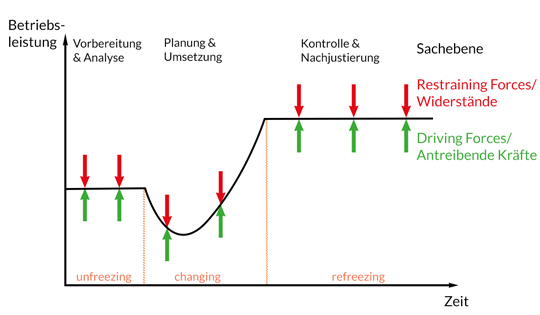
\includegraphics[width=0.7\textwidth]{3Phasen_Kurt_Lewin_web.jpg}
\end{frame}

\begin{frame}
\frametitle{Vorbereitung \& Analyse}\framesubtitle{Modell nach Kurt Levin}
\begin{itemize}
\item tritratrullala

\end{itemize}
\end{frame}


\end{document}
